% Created 2020-05-04 Mon 12:30
% Intended LaTeX compiler: pdflatex
\documentclass[11pt]{article}
\usepackage[utf8]{inputenc}
\usepackage[T1]{fontenc}
\usepackage{graphicx}
\usepackage{grffile}
\usepackage{longtable}
\usepackage{wrapfig}
\usepackage{rotating}
\usepackage[normalem]{ulem}
\usepackage{amsmath}
\usepackage{textcomp}
\usepackage{amssymb}
\usepackage{capt-of}
\usepackage{hyperref}
\usepackage{minted}
\usepackage{/home/ryan/Dropbox/profiles/Templates/LaTeX/ScreenStyle}
\usepackage[citestyle=numeric, bibstyle=numeric,hyperref=true,backref=true, maxcitenames=3,url=true,backend=biber,natbib=true]{biblatex}
\addbibresource{/home/ryan/Dropbox/Studies/Papers/references.bib}
%%% TeX-command-extra-options: "-shell-escape"
\author{Ryan Greenup}
\date{\today}
\title{Analysing Twitter for Ubisoft}
\hypersetup{
 pdfauthor={Ryan Greenup},
 pdftitle={Analysing Twitter for Ubisoft},
 pdfkeywords={},
 pdfsubject={},
 pdfcreator={Emacs 27.0.91 (Org mode 9.4)}, 
 pdflang={English}}
\begin{document}

\maketitle
\tableofcontents


\section{8.1 Analysing the Relationship Between Friends and Followers for Twitter Users}
\label{sec:org50dd8ed}
\subsection{8.1.1 Retrieve the posts from Twitter}
\label{sec:orge20fd44}
relevant posts can be retrieved from twitter by utilising the \texttt{rtweet} package, packages can be loaded for use in \textbf{\textbf{\uline{R}}} thusly:

\begin{listing}[htbp]
\begin{minted}[]{r}
# Load Packages -----------------------------------------------------------
setwd("~/Dropbox/Notes/DataSci/Social_Web_Analytics/SWA-Project/scripts/")

if (require("pacman")) {
  library(pacman)
} else{
  install.packages("pacman")
  library(pacman)
}

pacman::p_load(xts, sp, gstat, ggplot2, rmarkdown, reshape2,
               ggmap, parallel, dplyr, plotly, tidyverse,
               reticulate, UsingR, Rmpfr, swirl, corrplot,
               gridExtra, mise, latex2exp, tree, rpart,
               lattice, coin, primes, epitools, maps, clipr,
               ggmap, twitteR, ROAuth, tm, rtweet, base64enc,
               httpuv, SnowballC, RColorBrewer, wordcloud,
               ggwordcloud, tidyverse, boot)
\end{minted}
\caption{\label{org715e94c}Load the Packages for \textbf{\textbf{\emph{R}}}}
\end{listing}


The \texttt{rtweet} API will search for tweets that contain all the words of a query
regardless of uppercase or lowercase usage \cite{kearney2019}.

In order to leverage the \emph{Twitter} API it is necessary to use tokens provided through a \emph{Twitter} developer account:

\begin{listing}[htbp]
\begin{minted}[]{r}
# Set up Tokens ===========================================================

options(RCurlOptions = list(
  verbose = FALSE,
  capath = system.file("CurlSSL", "cacert.pem", package = "RCurl"),
  ssl.verifypeer = FALSE
))

setup_twitter_oauth(
  consumer_key = "*************************",
  consumer_secret = "**************************************************",
  access_token = "**************************************************",
  access_secret = "*********************************************"
)

# rtweet ==================================================================
tk <-    rtweet::create_token(
  app = "SWA",
  consumer_key    = "*************************",
  consumer_secret = "**************************************************",
  access_token    = "**************************************************",
  access_secret   = "*********************************************",
  set_renv        = FALSE
\end{minted}
\caption{\label{org2337af2}Import the twitter tokens (redacted)}
\end{listing}

and hence all tweets containing a mention of \emph{Ubisoft} can be returned and saved to disk as shown in listing \ref{orgd16643e}:

\begin{listing}[htbp]
\begin{minted}[]{r}
 n <- 1000
 tweets.company <- search_tweets(q = 'ubisoft', n = n, token = tk,
                                 include_rts = FALSE)
 save(tweets.company[,], file = "resources/Download_1.Rdata")
\end{minted}
\caption{\label{orgd16643e}Save the Tweets to the HDD as an \texttt{rdata} file}
\end{listing}

\subsection{8.2.2 Count of Followers and Friends}
\label{sec:orgfd5a188}
In order to identify the number of users that are contained in the \emph{tweets} the
\texttt{unique()} function can be used to return a vector of names which can then be passed as an index to the vector of counts as shown in listing \ref{orgebb9134}, this provides that 81.7\% of the tweets are by unique users.

\begin{listing}[htbp]
\begin{minted}[]{r}
(users <- unique(tweets.company$name)) %>% length()
x <- tweets.company$followers_count[duplicated(tweets.company$name)]
y <- tweets.company$friends_count[duplicated(tweets.company$name)]

## > [1] 817
\end{minted}
\caption{\label{orgebb9134}Return follower count of twitter posts}
\end{listing}


\subsection{8.1.3 Summary Statistics}
\label{sec:org2034e3a}
The average number of friends and followers from users who posted tweets mentioning \emph{Ubisoft} can be returned using the \texttt{mean()} as shown in listing \ref{orgf7af30e}
this provides that on average each user has 586 friends and 63,620 followers.

\begin{listing}[htbp]
\begin{minted}[]{r}
x<- rnorm(090)
y<- rnorm(090)
(xbar <- mean(x))
(ybar <- mean(y))

## > [1] 4295.195
## > [1] 435.9449
\end{minted}
\caption{\label{orgf7af30e}Determine the average number of friends and followers}
\end{listing}

\subsection{8.1.4 Above Average Followers}
\label{sec:orgd1e6ffa}
Each user can be compared to the average number of followers, by using a logical
operator on the vector (e.g. \texttt{y > ybar}), this will return an output of logical
values. \textbf{\emph{R}} will coerce logicals into 1/0 values meaning that the mean value
will return the proportion of \texttt{TRUE} responses as shown in listing \ref{org05224db}. This
provides that:

\begin{itemize}
\item 2.4\%  of the have identified have an above average \textbf{number of followers}.
\item 20.6\% of the users identified have an above average \textbf{number of friends}.
\end{itemize}

\begin{listing}[htbp]
\begin{minted}[]{r}
(px_hat <- mean(x>xbar))
(py_hat <- mean(y>ybar))

## > [1] 0.0244798
## > [1] 0.2729498
\end{minted}
\caption{\label{org05224db}Calculate the proportion of users with above average follower counts}
\end{listing}


\subsection{8.1.5 Bootstrap confidence intervals}
\label{sec:org4c8d06a}
\subsubsection{a/b.) Generate a bootsrap distribution}
\label{sec:org8537dc5}

A bootstrap assumes that the population is an infinitely large repetition of the
sample and may be produces with respect to follower counts by resampling with
replacement/repetition and plotted using the \texttt{ggplot2} library as deomonstrated
in listings \ref{org1f37fd8} and \ref{org10c35ec} and shown in figure \ref{fig:orgfa96dc0}.

This shows that the population follower counts is a non-normal skew-right
distribution, which is expected because the number of friends is an integer value bound by zero \cite{nist2013}.

\begin{listing}[htbp]
\begin{minted}[]{r}
## Resample the Data
(bt_pop <- sample(x, size = 10^6, replace = TRUE)) %>% head()

## > [1]   7 515 262 309 186 166
\end{minted}
\caption{\label{org1f37fd8}Bootstrapping a population from the sample.}
\end{listing}

\begin{listing}[htbp]
\begin{minted}[]{r}
## Make the Population
bt_pop_data <- tibble("Followers" = bt_pop)
ggplot(data = bt_pop_data, aes(x = Followers)) +
  geom_histogram(aes(y = ..density..), fill = "lightblue", bins = 35, col = "pink") +
  geom_density(col = "violetred2") +
  scale_x_continuous(limits = c(1, 800)) +
  theme_bw() +
  labs(x = "Number of Followers", y = "Density",
       title = "Bootstrapped population of Follower Numbers")

\end{minted}
\label{org10c35ec}
\end{listing}

\begin{figure}[htbp]
\centering
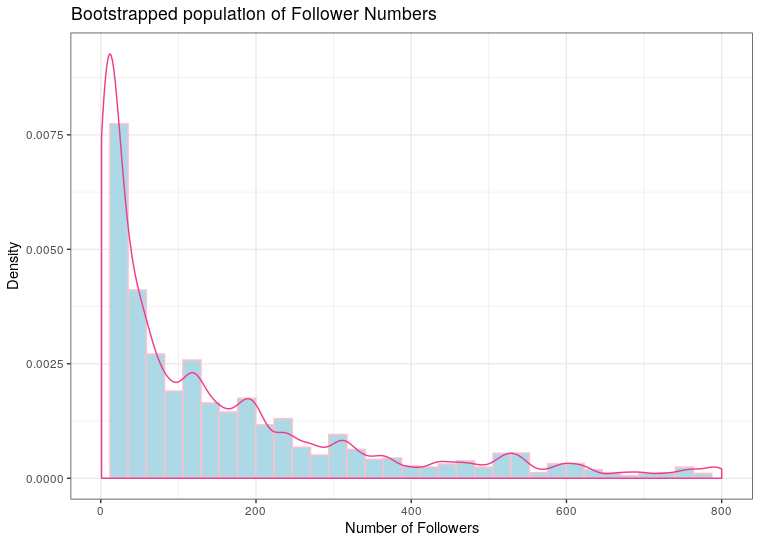
\includegraphics[width=12cm]{./Figures/BootStrap_Pop.png}
\caption{\label{fig:orgfa96dc0}Histogram of the bootrapped population of follower counts}
\end{figure}

\subsubsection{c.) Estimate a Confidence Interval for the population mean Follower Counts}
\label{sec:org353bada}
In order to perform a bootrap for the population mean value of follower counts it is necessary to:

\begin{enumerate}
\item Resample the data with replacement
\begin{itemize}
\item i.e. randomly select values from the sample allowing for repetition
\end{itemize}
\item Measure the statistic of concern
\item Replicate this a sufficient number of times
\begin{itemize}
\item i.e. Greater than or equal to 1000 times \cite[Ch. 5]{davison1997}
\end{itemize}
\end{enumerate}

This is equivalent to drawing a sample from a population that is infinitely large and constructed of repetitions of the sample. This can be performed in \textbf{\emph{R}} as shown in listing \ref{orge1a3255}.


\begin{listing}[htbp]
\begin{minted}[]{r}
xbar_boot_loop <- replicate(10^3, {
  s <- sample(x, replace = TRUE)
  mean(s)
  })
quantile(xbar_boot_loop, c((1-0.97)/2, (1+0.97)/2))

##       1.5%      98.5%
##   588.4189 10228.7352
\end{minted}
\caption{\label{orge1a3255}Confidence Interval of Mean Follower Count in Population}
\end{listing}

A 97\% probability interval is such that a sample drawn from a population will contain the population mean in that interval 97\% of the time, this means that it may be concluded with a high degree of certainty that the true population mean lies between 588 and 10228.

\begin{enumerate}
\item Alternative Approaches
\label{sec:org59c6c86}
If this data was normally distributed it may have been appropriate to consider
bootstrapping the standard error and using a \(t\) distribution, however it is more appropriate to use a
percentile interval for skewed data such as this, in saying that however this method is not considered to be very accurate in the literature and is often too narrow. \cite[Section 4.1]{hesterberg2015}

\begin{itemize}
\item It's worth noting that the normal \(t\) value bootstrap offers no advantage over
using a \(t\) distribution (other than being illustrative of bootstrapping
generally) \cite[Section 4.1]{hesterberg2015}
\end{itemize}


 The \texttt{boot} package is a bootstrapping library common among authors in the data science sphere
 \cite[p. 295]{james2013} \cite[p. 237]{wiley2019} that implements
 confidence intervals consistent with work by Davison and Hinkley
 \cite{ripley2020} in there texbook \emph{Bootstrap Methods and their Application}.
In this work it is provided that the \(BC_{a}\) method of constructing confidence
 intervals is  superior to mere percentile
 methods in terms of accuracy \cite[Ch. 5]{davison1997}, a sentiment echoed in the literature. \cite[Ch. 5]{carpenter2000,davison1997}

Such methods can be implemented in \textbf{\emph{R}} by passing a function to the the \texttt{boot} call as shown in listing \ref{org77a75dc}. This provides a broader interval, providing that the true confidence interval could lie between 1079 and 16227 followers.

\begin{listing}[htbp]
\begin{minted}[]{r}
xbar_boot <- boot(data = x, statistic = mean_val, R = 10^3)
boot.ci(xbar_boot, conf = 0.97, type = "bca", index = 1)

## BOOTSTRAP CONFIDENCE INTERVAL CALCULATIONS
## Based on 1000 bootstrap replicates
##
## CALL :
## boot.ci(boot.out = xbar_boot, conf = 0.97, type = "bca", index = 1)
##
## Intervals :
## Level       BCa
## 97%   ( 1079, 16227 )
## Calculations and Intervals on Original Scale
## Warning : BCa Intervals used Extreme Quantiles
## Some BCa intervals may be unstable
## Warning message:
## In norm.inter(t, adj.alpha) : extreme order statistics used as endpoints
\end{minted}
\caption{\label{org77a75dc}Bootstrap of population mean follower count implementing the \(BC_{a}\) method}
\end{listing}

\label{org03950ae}
\bibliography{references}

\label{orgfc5f6ea}
 \bibliographystyle{unsrt}
\end{enumerate}

\subsubsection{d.) Estimate a Confidence Interval for the population mean Friend Counts}
\label{sec:org118849d}
A Confidence interval for the population mean friend counts may be constructed in a like wise fashion as shown in listings \ref{org27e706b}. This provides that the 97\% confidence interval for the population mean friend count is between 384 and 502 (or 387 and 496 if the \(BC_{a}\) method used, they're quite close and so the more conservative percentile method will be accepted).

\begin{listing}[htbp]
\begin{minted}[]{r}
# d.) Estimate a Confidence Interval for the populattion mean Friend Count ===
# Using a Percentile Method #####################################################
ybar_boot_loop <- replicate(10^3, {
  s <- sample(y, replace = TRUE)
  mean(s)
  })
quantile(ybar_boot_loop, c(0.015, 0.985)

# Using BCA Method #############################################################
mean_val <- function(data, index) {
  X = data[index]
  return(mean(X))
}

xbar_boot <- boot(data = y, statistic = mean_val, R = 10^3)
boot.ci(xbar_boot, conf = 0.97, type = "bca", index = 1)


##     1.5%    98.5%
## 383.7619 501.5903
##
## BOOTSTRAP CONFIDENCE INTERVAL CALCULATIONS
## Based on 1000 bootstrap replicates
##
## CALL :
## boot.ci(boot.out = xbar_boot, conf = 0.97, type = "bca", index = 1)
##
## Intervals :
## Level       BCa
## 97%   (386.8, 496.7 )
## Calculations and Intervals on Original Scale
## Some BCa intervals may be unstable
\end{minted}
\caption{\label{org27e706b}Bootstrap of population mean follower count}
\end{listing}

\subsection{{\bfseries\sffamily FIXME} 8.1.6 Estimate a 97\% Confidence Interval for the High Friend Count Proportion}
\label{sec:org2b3ece7}
In order to bootstrap a confidence interval for the proportion of users with
above average follower counts, repeteadly draw random samples from an infinitely
large population composed entirely of the sample, and record the sampled
proportion. this can be acheived by resampling the observations of above and
below as shown in listing \ref{org070fe29}.

This provides that:
\begin{itemize}
\item The 97\% confidence interval for the population proportion of users that have an above average number of friends is between 0.24 and 0.31.
\begin{itemize}
\item i.e. The probability of any given sample containing the population mean within this interval would be 97\%, although  that doesn't however mean that there is a 97\% probability that this interval contains the value, merely that we may be 97\% \emph{confident}
\end{itemize}
\end{itemize}

\begin{listing}[htbp]
\begin{minted}[]{r}
# 8.1.6 High Friend Count Proportion -------------------------------------------
prop <- factor(c("Below", "Above"))
## 1 is above average, 2 is below
py_hat_bt <- replicate(10^3, {
  rs      <- sample(c("Below", "Above"),
                    size = length(y),
                    prob = c(py_hat, 1-py_hat),
                    replace = TRUE)
isabove <- rs == "Above"
mean(isabove)
})
quantile(py_hat_bt, c(0.015, 0.985))


##      1.5%     98.5%
## 0.2399021 0.3072215
## > > > . + > > >
## BOOTSTRAP CONFIDENCE INTERVAL CALCULATIONS
## Based on 1000 bootstrap replicates
##
## CALL :
## boot.ci(boot.out = py_hat_boot, conf = 0.97, type = "bca")
##
## Intervals :
## Level       BCa
## 97%   ( 0.2399,  0.3072 )
## Calculations and Intervals on Original Scale
\end{minted}
\caption{\label{org070fe29}Bootstrap of Proportion of Friends above average}
\end{listing}
\subsection{8.1.7 Is the Number of Friends Independent to the Number of Followers}
\label{sec:org9678d37}
One method to determine whether or not the number of followers is independent of the number of friends is to bin the counts and determine whether or not the distribution of users across those counts is consistent with the hypothesis of independence.

\subsubsection{Bin the Follower and Friend Categories}
\label{sec:orgc26cd1e}
The counts may be binned by performing a logical interval test as shown in listing \ref{orge2d8eb5}.

\begin{listing}[htbp]
\begin{minted}[]{r}
## Assign Categories
x_df <- data.frame(x)
x_df$cat[0       <= x_df$x & x_df$x < 100] <- "Tens"
x_df$cat[100     <= x_df$x & x_df$x < 1000] <- "Hundreds"
x_df$cat[1000    <= x_df$x & x_df$x < 2000] <- "1Thousands"
x_df$cat[2000    <= x_df$x & x_df$x < 3000] <- "2Thousands"
x_df$cat[3000    <= x_df$x & x_df$x < 4000] <- "3Thousands"
x_df$cat[4000    <= x_df$x & x_df$x < 5000] <- "4Thousands"
x_df$cat[5000    <= x_df$x & x_df$x < Inf] <- "5ThousandOrMore"

### Make a factor
x_df$cat <- factor(x_df$cat, levels = var_levels, ordered = TRUE)

### Determine Frequencies
(x_freq <- table(x_df$cat) %>% as.matrix())

## ** b) Find the Friend Count Frequency ===========================================
## Assign Categories
y_df <- data.frame(y)
y_df$cat[0       <= y_df$y & y_df$y < 100] <- "Tens"
y_df$cat[100     <= y_df$y & y_df$y < 1000] <- "Hundreds"
y_df$cat[1000    <= y_df$y & y_df$y < 2000] <- "1Thousands"
y_df$cat[2000    <= y_df$y & y_df$y < 3000] <- "2Thousands"
y_df$cat[3000    <= y_df$y & y_df$y < 4000] <- "3Thousands"
y_df$cat[4000    <= y_df$y & y_df$y < 5000] <- "4Thousands"
y_df$cat[5000    <= y_df$y & y_df$y < Inf]  <- "5ThousandOrMore"

### Make a factor
y_df$cat <- factor(y_df$cat, levels = var_levels, ordered = TRUE)

### Determine Frequencies
(y_freq <- table(y_df$cat) %>% as.matrix())
\end{minted}
\caption{\label{orge2d8eb5}Use Logical Test to Assign observations into bins}
\end{listing}

\subsubsection{Find the Group frequency}
\label{sec:orgd17fe3d}
These values may be tabluated in order to count the occurence of users among these categories as shown in listing \ref{org9026364} and table \ref{tab:orgda60606}.

\begin{listing}[htbp]
\begin{minted}[]{r}
vals <- t(cbind(x_freq, y_freq))
rownames(vals) <- c("Followers.x", "followers.y")
vals

##             Tens Hundreds 1Thousands 2Thousands 3Thousands 4Thousands
## Followers.x  421      317         39         11          9          2
## followers.y  262      476         47         15          6          9
##             5ThousandOrMore
## Followers.x              18
## followers.y               2
\end{minted}
\caption{\label{org9026364}Tabulate the binned counts for the distribution of users among among amount and status.}
\end{listing}

\begin{table}[htbp]
\caption{\label{tab:orgda60606}Table of Binned Friend and Follower counts, transposed relative to code.}
\centering
\begin{tabular}{lrr}
 & \textbf{\textbf{\emph{Followers}}} & \textbf{\textbf{\emph{Friends}}}\\
\emph{Tens} & 421 & 262\\
\emph{Hundreds} & 317 & 476\\
\emph{1 - Thousands} & 39 & 47\\
\emph{2 - Thousands} & 11 & 15\\
\emph{3 - Thousands} & 9 & 6\\
\emph{4 - Thousands} & 2 & 9\\
\emph{5 Thousand or More} & 18 & 2\\
\end{tabular}
\end{table}

\subsubsection{Find the Expected Counts under each group and test for independence}
\label{sec:org7cd3cd8}
The expected count of each cell, under the assumption that the two metrics are
independent, will be the proportion users per bracket multiplied by the number
of users in that status group. This implies that any cell will be:

\begin{itemize}
\item the product of the row sum, multiplied by the column sum divided by the number of counts.
\end{itemize}

This can be equivalently expressed as an outer product as shown in equation
\eqref{eq:1}, in \textbf{\emph{R}} this operation is denoted by the \texttt{\%o\%} operator, which is
shorthand for the \texttt{outer()} function, this and other summary statistics may be
evaluated as shown in listing \ref{org61a3b24}.

The outer product is such that:


$$
\mathbf{u} \otimes \mathbf {v} =\mathbf {u} \mathbf {v} ^{\textsf {T}}={\begin{bmatrix}u_{1}\\u_{2}\\u_{3}\\u_{4}\end{bmatrix}}{\begin{bmatrix}v_{1}&v_{2}&v_{3}\end{bmatrix}}={\begin{bmatrix}u_{1}v_{1}&u_{1}v_{2}&u_{1}v_{3}\\u_{2}v_{1}&u_{2}v_{2}&u_{2}v_{3}\\u_{3}v_{1}&u_{3}v_{2}&u_{3}v_{3}\\u_{4}v_{1}&u_{4}v_{2}&u_{4}v_{3}\end{bmatrix}}.
$$

This means the matrix of expected frequencies can be expressed as an outer product thusly:

\begin{align}
\label{eq:orgb8b4beb}
\mathbf{\vec{e}}= \frac{1}{n} \times \begin{bmatrix} \sum^{n}_{j= 1} \left[ o_{1j} \right] \\  \sum^{n}_{j= 1}
\left[ o_{2j} \right]  \\ \sum^{n}_{j= 1} \left[ o_{3j} \right]   \\
\sum^{n}_{j= 1} \left[ o_{4j} \right]  \\ \vdots  \\
\sum^{n}_{j= 1} \left[ o_{nj} \right]     \end{bmatrix} 
\begin{bmatrix}  \sum^{n}_{j= 1} \left[ o_{i1}  \right] \\  \sum^{n}_{j= 1}
\left[ o_{i2}  \right] \\ \sum^{n}_{j= 1} \left[ o_{i3}  \right] \\ \cdots \\
\sum^{n}_{j= 1} \left[ o_{in}  \right]   \end{bmatrix}  ^{\normalsize \mathrm{T}} \label{eq:1}
\end{align}

\begin{listing}[htbp]
\begin{minted}[]{r}
## ***** Calculate Summary Stats
n <- sum(vals)
bracket_prop <- colSums(vals) / n
metric_prop  <- rowSums(vals) / n
o <- vals
e <- rowSums(vals) %o% colSums(vals) / n
chi_obs <- sum((e-o)^2/e)
\end{minted}
\caption{\label{org61a3b24}Calculate Expected frequency of values under the assumption of independence.}
\end{listing}

\begin{enumerate}
\item Testing Independence
\label{sec:org9524a09}
In order to test whether or not the distribution of users among brackets is
independent of being a follower or friend a \(\chi^{2}\) test may be used, this
can be evaluated from a model or simulated, in \textbf{\emph{R}}, the simulated test is
shown in listing \ref{org0909011}, this provides a \(p\) -value < 0.0005, which means that the hypothesis of independence may be rejected with a high degree of certainty.

\begin{listing}[htbp]
\begin{minted}[]{r}
chisq.test(vals, simulate.p.value = TRUE)


## 	Pearson's Chi-squared test with simulated p-value (based on 2000
## 	replicates)
##
## data:  vals
## X-squared = 88.109, df = NA, p-value = 0.0004998
\end{minted}
\caption{\label{org0909011}Chi-Square testing for independence between friend and follower bin categories.}
\end{listing}

\begin{enumerate}
\item From First Principles
\label{sec:org3123fa2}
The \(\chi^{2}\) statistic may be performed from first principles by randomly
sampling the values at the rate at which they occured, tabulating those counts, measuring the \(\chi^{2}\) -value and then repeating this many times.

Because the samples are random they must be independent and average number of
positives is hence an estimate for the \emph{FPR}, which is in turn an estimate for
the \(p\) -value. This technique is demonstrated in listing \ref{org17f909d}, the p-value
being returned as 0.0004, this value is consistent with the value produced by
\textbf{\emph{R}}'s built in \texttt{chisq.test} function and so is accepted.

\begin{listing}[htbp]
\begin{minted}[]{r}
## ***** Create Vectors of factor levels
brackets <- unique(x_df$cat)
metrics <- c("follower", "friend")

## ***** Simulate the data Assuming H_0
## I.e. assuming that the null hypothesis is true in that
## the brackets assigned to followers are independent of the friends
## (this is a symmetric relation)

s <- replicate(10^4,{
  ## Sample the set of Metrics
  m <- sample(metrics, size = n, replace = TRUE, prob = metric_prop)

  ## Sample the set of Brackets (i.e. which performance bracket the user falls in)
  b <- sample(brackets, size = n, replace = TRUE, prob = bracket_prop)

  ## Make a table of results
  o <- table(m, b)
  o

  ## Find What the expected value would be
  e_sim <- t(colSums(e) %o% rowSums(e) / n)

  ## Calculate the Chi Stat
  chi_sim <- sum((e_sim-o)^2/e_sim)
  chi_sim

  ## Is this more extreme, i.e. would we reject null hypothesis?
  chi_sim > chi_obs

})

mean(s)
\end{minted}
\caption{\label{org17f909d}Performing a \(\chi^{2}\) statistic from first principles}
\end{listing}
\end{enumerate}
\end{enumerate}
\subsubsection{{\bfseries\sffamily FIXME} Conclusion}
\label{sec:org6953fa5}
The \(p\) -value measures the probability of rejecting the null hypothesis when it is true, i.e. the probability of a detecting a \emph{false positive}, a very small \(p\) -value is hence good evidence that the null hypothesis should be rejected (because doing so would unlikely to be a mistake).

In saying that however the \(p\) -value is distinct from the \emph{power} statistic, which is a measure of \emph{/the probability of accepting the alternative hypothesis} when it is true, a low \(p\) -value is not a measurement of the probability of being correct.

Hence me way conclude, with a high degree of certainty, that the follower and friend counts are not independent of one another.
\section{8.2 Finding Themes in tweets}
\label{sec:orgace71d9}



\begin{quote}
In order to clean the corpus it will be necessary to:

\begin{enumerate}
\item remove numbers
\item remove punctuation
\item remove whitespace
\item case fold all characters to lower case
\item remove a set of stop words
\item reduce each word to its stem
\end{enumerate}
\end{quote}
\subsection{Should Emoji's be removed}
\label{sec:org9920ddd}
These studies suggest that

Emoji's are variables that can be used as a predictive features \cite{lecompte2017}  and can improve the performance of Sentiment Analysis Models \cite{shiha2017} that use the \emph{Bag of Words Approach}
\subsection{8.2.8 Find Users with Above Average Friend Counts}
\label{sec:orgc17bae0}
Users with Above average Friend Counts can be identified by filtering the tweets
data frame for two conditions:

\begin{enumerate}
\item non-duplicated \texttt{user-id}
\item \texttt{friend\_count} greater than average
\end{enumerate}

This can be acheived easily using the \texttt{dplyr} package as shown in \ref{org5f322ed}, these users are shown in the appendix in table \ref{tab:org0d93e6b}.

\begin{listing}[htbp]
\begin{minted}[]{r}
select <- dplyr::select
filter <- dplyr::filter
interested_vars <- c("user_id", "friends_count")
(friend_counts <- tweets.company %>%
  select(interested_vars) %>%
  filter(!duplicated(user_id)))

(high_friends <- friend_counts %>%
  filter(friends_count > mean(friends_count, na.rm = TRUE)))

## Export Friends List
write.csv(high_friends[order(
  high_friends$friends_count,
  decreasing = TRUE),], file = "/tmp/highfriend.csv")
\end{minted}
\caption{\label{org5f322ed}Use \texttt{dplyr} to Filter for Users with a high Friend Count}
\end{listing}





\section{Appendix}
\label{sec:org793023a}
\subsection{Users with High Friend Count}
\label{sec:orgf976018}

\begin{table}[htbp]
\caption{\label{tab:org0d93e6b}User ID and Friend Count of users with above highest friend count in sample}
\centering
\begin{tabular}{llr}
``'' & \textbf{\emph{User ID}} & \textbf{\emph{Friend Count}}\\
``1'' & ``274488119'' & 8752\\
``2'' & ``743771665'' & 5002\\
``3'' & ``1036014247'' & 4999\\
``4'' & ``2281452613'' & 4992\\
``5'' & ``1554453560'' & 4958\\
``6'' & ``981233818408570880'' & 4944\\
``7'' & ``931765564388921344'' & 4836\\
``8'' & ``807405140'' & 4710\\
``9'' & ``1112579152970842112'' & 4514\\
``10'' & ``2441577446'' & 4322\\
``11'' & ``552692862'' & 4229\\
``12'' & ``956297007127252992'' & 3976\\
``13'' & ``22493896'' & 3675\\
``14'' & ``255922782'' & 3500\\
``15'' & ``1067409881332936709'' & 3312\\
``16'' & ``27998570'' & 3210\\
``17'' & ``715118521555017728'' & 3099\\
``18'' & ``2356170174'' & 2885\\
``19'' & ``2372688230'' & 2880\\
``20'' & ``1868357425'' & 2719\\
\end{tabular}
\end{table}
\end{document}
